\chapter{Исследовательская часть}

\section{Цель исследования}

Целью исследования является сравнение эффективности трёх алгоритмов умножения матриц: стандартного, алгоритма Винограда и оптимизированного алгоритма Винограда.  
Для анализа производительности выполнены замеры времени работы алгоритмов при различных размерах матриц в двух режимах:
\begin{itemize}
	\item \textbf{худший случай} — матрицы нечётного размера;
	\item \textbf{лучший случай} — матрицы чётного размера.
\end{itemize}

\section{Худший случай}

График зависимости времени работы алгоритмов от размера матрицы в худшем случае приведён на рисунке~\ref{fig:worst}.

\begin{figure}[H]
	\centering
	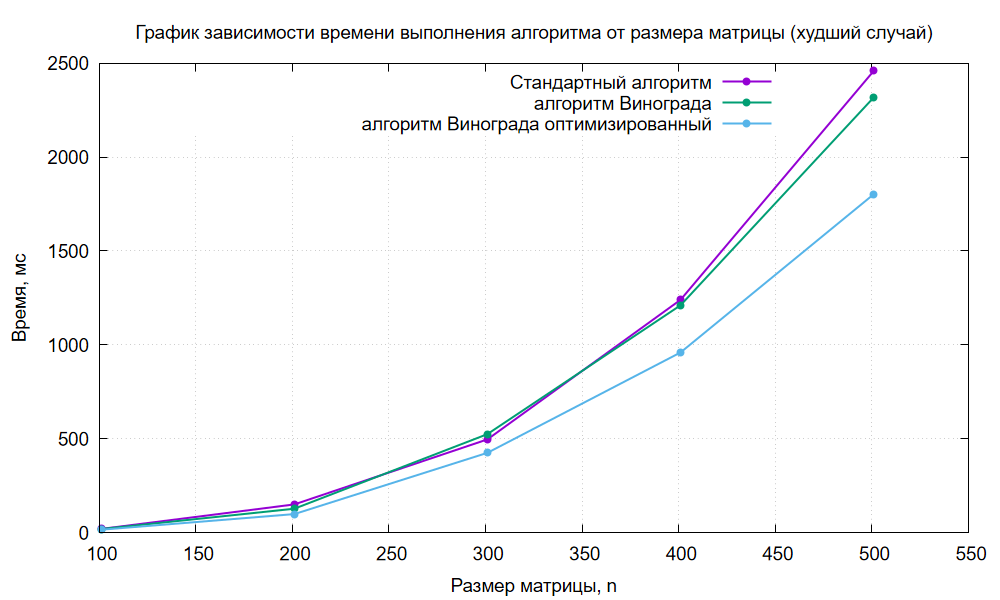
\includegraphics[width=0.85\linewidth]{benchmark_worst.png}
	\caption{Сравнение алгоритмов умножения матриц (худший случай)}
	\label{fig:worst}
\end{figure}

В таблице~\ref{tab:worst} приведены результаты замеров времени работы трёх алгоритмов при умножении квадратных матриц нечётного размера.

\begin{table}[H]
	\centering
	\caption{Результаты замеров времени (в миллисекундах) для худшего случая}
	\label{tab:worst}
	\begin{tabular}{|c|c|c|c|}
		\hline
		Размер $n$ & Стандартный алгоритм & Алгоритм Винограда & Оптимизированный Виноград \\
		\hline
		101 & 15.06 & 13.78 & 10.93 \\
		201 & 116.48 & 107.50 & 85.38 \\
		301 & 387.57 & 355.84 & 282.34 \\
		401 & 930.25 & 851.76 & 670.05 \\
		501 & 1800.02 & 1636.03 & 1299.95 \\
		\hline
	\end{tabular}
\end{table}

\section{Лучший случай}

В таблице~\ref{tab:best} приведены результаты замеров времени работы трёх алгоритмов при умножении квадратных матриц чётного размера.

График зависимости времени работы алгоритмов от размера матрицы в лучшем случае приведён на рисунке~\ref{fig:best}.

\begin{figure}[H]
	\centering
	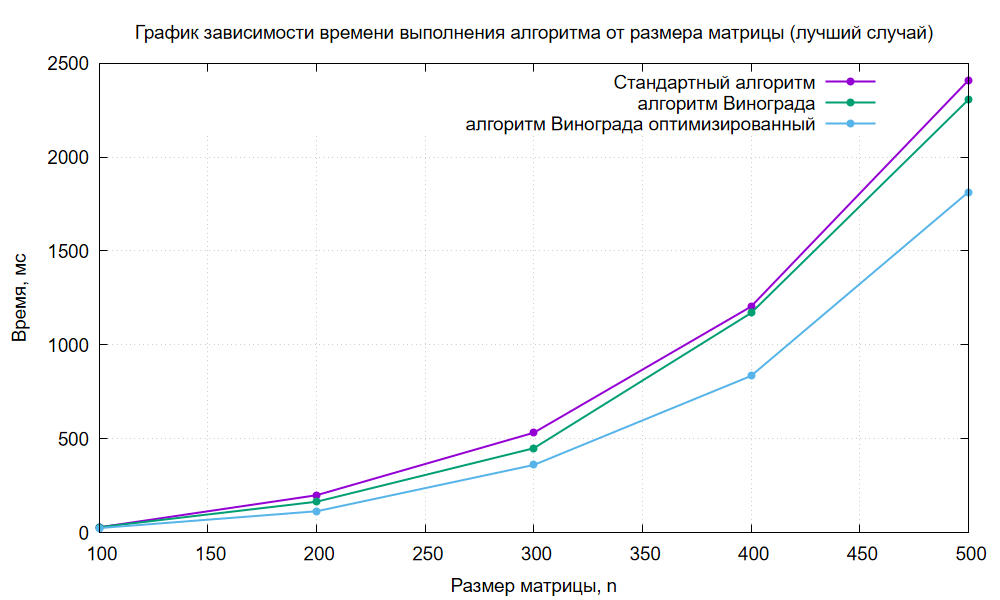
\includegraphics[width=0.85\linewidth]{benchmark_best.png}
	\caption{Сравнение алгоритмов умножения матриц (лучший случай)}
	\label{fig:best}
\end{figure}

\begin{table}[H]
	\centering
	\caption{Результаты замеров времени (в миллисекундах) для лучшего случая}
	\label{tab:best}
	\begin{tabular}{|c|c|c|c|}
		\hline
		Размер $n$ & Стандартный алгоритм & Алгоритм Винограда & Оптимизированный Виноград \\
		\hline
		100 & 14.25 & 13.41 & 10.34 \\
		200 & 114.41 & 104.30 & 82.89 \\
		300 & 386.43 & 354.84 & 281.87 \\
		400 & 920.57 & 850.07 & 669.74 \\
		500 & 1818.12 & 1637.69 & 1293.03 \\
		\hline
	\end{tabular}
\end{table}

Для чётных размеров матриц эффективность алгоритма Винограда достигает максимума благодаря полному использованию парных индексов.

Расхождения между теоретическими и данными, полученными программным путём находятся в допустимых пределах и объясняются аппаратными особенностями тестовой системы.


\section*{Вывод}

Результаты исследований подтверждают сделанные теоретические выводы:
\begin{itemize}
	\item наименьшее время выполнения демонстрирует оптимизированный алгоритм Винограда;
	\item базовая версия метода Винограда в среднем быстрее классического способа, но уступает оптимизированной;
	\item наблюдается зависимость времени работы от чётности размеров матриц: при нечётных размерах производительность незначительно снижается.
\end{itemize}

\clearpage
